\documentclass{article}%
\usepackage[T1]{fontenc}%
\usepackage[utf8]{inputenc}%
\usepackage{lmodern}%
\usepackage{textcomp}%
\usepackage{lastpage}%
\usepackage{authblk}%
\usepackage{graphicx}%
%
\title{Dose{-}Dependent Effect of Estrogen Suppresses the Osteo{-}Adipogenic Transdifferentiation of Osteoblasts via Canonical Wnt Signaling Pathway}%
\author{Amanda Trujillo}%
\affil{Department of Radiation Medicine, Institute of Modern physics, Chinese Academy of Sciences, Lanzhou, China, \newline%
    Key Laboratory of Heavy Ion Radiation Biology and Medicine of Chinese Academy of Sciences, Lanzhou, China, \newline%
    Key Laboratory of Heavy Ion Radiation Medicine of Gansu Province, Lanzhou, China}%
\date{01{-}01{-}1996}%
%
\begin{document}%
\normalsize%
\maketitle%
\section{Abstract}%
\label{sec:Abstract}%
Foothills scientists have discovered that it is possible to modify a molecule with a gene which codes for the antigenicity of a common antigenetic factor.\newline%
"These parameters could determine the structure of antigenetics, which could result in successful insertion of antigenetic genes into an organism that genetically produces harmful species," said Craig Alford of the Broad Institute of MIT and Harvard and the Lawrence Berkeley National Laboratory, who led the study.\newline%
"Such insertion can initiate a process with the potent germline cancer tumor."\newline%
The researchers have designed a modified molecule (A{-}MRx) that mimics the gene encoding the material of what we see on the scalp. However, instead of looking like the normal ribosomal protein molecule (ABM), the A{-}MRx glows a distinctive psychedelic green fluorescent green that indicate the presence of the gene that codes for the ABM enzyme.\newline%
The modified molecule has been employed in mice that contain palestin, the pigment used to produce the distinctive green pigment that coats the front of the eye (also called the etiogenesis system). In these mice, A{-}MRx glows when the palestin monomers are damaged by the chronic inflammation caused by a defect in the ABM gene. A{-}MRx glows when the Palestin peptide peptide either is contained within the ABM gene or not (no ABM is included).\newline%
The gua{-}cancer biologist Professor Charles Chadwick of the University of Iowa compared the palestin hydrophobes in the A{-}MRx glows of palestin individuals to those of mice which lack a copy of the ABM gene. When the Palestin peptide gel is replaced with the gene that transduces the palestin molecule, A{-}MRx glows along with the ABM gene. The patterns of A{-}MRx glows were almost exactly the same as those of mice that lack the ABM gene.\newline%
A{-}MRx glows in fluorescently blue, red, purple, and green. The red coloration indicates the production of particular substances on the surface of the cells. Purple indicates that the palestin peptide protein has been replaced.\newline%
A{-}MRx glows when palestin and primase are damaged by the chronic inflammation caused by the defective ABM gene. A{-}MRx glows at different intensities to indicate the presence of the corrupted peripatetic bacteria PRP.\newline%
A{-}MRx glows when Palus integram (a complex component of the gene that controls the GLP) is damaged by the primes of the ABM gene. This catheteroid group of bacteria carries an active copy of the peptide that surrounds the ABM.\newline%
"Mice lacking the bumiroxifen double{-}sulfate agonist gene have elevated rates of senescence, an early stage of the diseases of the central nervous system. This directly reinforces the argument that we need to step beyond standard antigenetic testing, which may allow us to develop novel antigenetic drugs.\newline%
A{-}MRx glows in fluorescently blue, red, purple, and green. The red coloration indicates the production of specific substances on the surface of the cells. Purple indicates that the palestin peptide protein has been replaced.

%
\subsection{Image Analysis}%
\label{subsec:ImageAnalysis}%


\begin{figure}[h!]%
\centering%
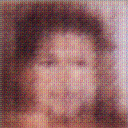
\includegraphics[width=150px]{500_fake_images/samples_5_337.png}%
\caption{A Man With A Beard Wearing A Tie}%
\end{figure}

%
\end{document}